\documentclass[12pt,letterpaper]{article}
\usepackage[utf8]{inputenc}
\usepackage[spanish]{babel}
\usepackage[T1]{fontenc}
\usepackage{bookman}
\usepackage{makeidx}
\usepackage{amsmath}
\usepackage{amsfonts}
\usepackage{amssymb}
\usepackage{listings}
\usepackage{cite}
\usepackage{graphicx}
\usepackage{subfig}
\usepackage{float}
\usepackage{ragged2e}
\graphicspath{ {imagenes/} }
\usepackage[left=2.5cm,right=2.5cm,top=3cm,bottom=3cm]{geometry}
\title{Reporte primer bloque de Programas}
\author{Javier Said Naranjo Miranda}


\begin{document}

\begin{titlepage}
\centering
	{\LARGE Instituto Polit\'ecnico Nacional \par}
	\vspace{1cm}
	{\Large Escuela Superior de C\'omputo \par}	
	\vspace{1.5cm}
	{\large Teor\'ia Computacional \par}
	\vspace{1cm}
	{\Large Reporte segundo bloque de programas \par}
	\vspace{1.5cm}
	{\Large\itshape Alumno: Javier Said Naranjo Miranda \par}
	\vfill
	Grupo: 2CM4 \par
	\vfill	
	\newpage
	

\end{titlepage}
\raggedright
\tableofcontents
\newpage
\section{Automata Web-Ebay}
\subsection{ Descripci\'on del programa}
\justify
El siguiente programa reconoce todas las palabras que contengan web o ebay,esto se realizar por medio de un automata finito determinista, podr\'a reconocer las palabras solo en textos en ingl\'es.\\
Consta de un modo autom\'atico y manual, ademas se podr\'a visualizar el diagrama del aut\'omata.\\
El programa guarda todas las palabras que encontr\'o y las guarda en un archivo de texto indicando el numero de fila y palabra en la que se encuentra.\\
\subsection{C\'odigo}
El c\'digo utilizado para la resoluci\'on del problema se muestra a continuaci\'on:\\

C\'odigo: webay.py
\lstset{language=Python, breaklines=true, basicstyle=\footnotesize}
\begin{lstlisting}[frame=single]
def automataWebay(caracter,estado,archivo):
	if(estado==0):
		estado=estadoCero(caracter,archivo)
	elif(estado==1):
		estado=estadoUno(caracter,archivo)
	elif(estado==2):
		estado=estadoDos(caracter,archivo)
	elif(estado==3):
		estado=estadoTres(caracter,archivo)
	elif(estado==4):
		estado=estadoCuatro(caracter,archivo)
	elif(estado==5):
		estado=estadoCinco(caracter,archivo)
	elif(estado==6):
		estado=estadoSeis(caracter,archivo)
	elif(estado==7):
		estado=estadoSiete(caracter,archivo)

	return estado

def estadoCero(caracter,archivo):
	if (caracter=='w'):
		archivo.write('q0--w-->q1\t')
		return 1
	elif (caracter=='e'):
		archivo.write('q0--e-->q4\t')
		return 4
	else:
		archivo.write('q0--%s-->q0\t' %caracter)
		return 0

def estadoUno(caracter,archivo):
	if(caracter=='w'):
		archivo.write('q1--w-->q1\t')
		return 1
	elif(caracter=='e'):
		archivo.write('q1--e-->q2\t')
		return 2
	else:
		archivo.write('q1--%s-->q0\t' % caracter)
		return 0

def estadoDos(caracter,archivo):
	if(caracter=='w'):
		archivo.write('q2--w-->q1\t')
		return 1
	elif(caracter=='e'):
		archivo.write('q2--e-->q4\t')
		return 4
	elif(caracter=='b'):
		archivo.write('q2--b-->q3\t')
		return 3
	else:
		archivo.write('q2--%s-->q0\t' % caracter)
		return 0

def estadoTres(caracter,archivo):
	if(caracter=='w'):
		archivo.write('q3--w-->q1\t')
		return 1
	elif(caracter=='e'):
		archivo.write('q3--e-->q4\t')
		return 4
	elif(caracter=='a'):
		archivo.write('q3--a-->q6\t')
		return 6
	else:
		archivo.write('q3--%s-->q0\t' % caracter)
		return 0

def estadoCuatro(caracter,archivo):
	if(caracter=='w'):
		archivo.write('q4--2-->q1\t')
		return 1
	elif(caracter=='e'):
		archivo.write('q4--e-->q4\t')
		return 4
	elif(caracter=='b'):
		archivo.write('q4--b-->q5\t')
		return 5
	else:
		archivo.write('q4--%s-->q0\t' % caracter)
		return 0

def estadoCinco(caracter,archivo):
	if(caracter=='w'):
		archivo.write('q5--w-->q1\t')
		return 1
	elif(caracter=='e'):
		archivo.write('q5--e-->q4\t')
		return 4
	elif(caracter=='a'):
		archivo.write('q5--a-->q6\t')
		return 6
	else:
		archivo.write('q5--%s-->q0\t' % caracter)
		return 0

def estadoSeis(caracter,archivo):
	if(caracter=='w'):
		archivo.write('q6--w-->q1\t')
		return 1
	elif(caracter=='e'):
		archivo.write('q6--e-->q4\t')
		return 4
	elif(caracter=='y'):
		archivo.write('q6--y-->q7\t')
		return 7
	else:
		archivo.write('q6--%s-->q0\t' % caracter)
		return 0

def estadoSiete(caracter,archivo):
	if(caracter=='w'):
		archivo.write('q7--w-->q1\t')
		return 1
	elif(caracter=='e'):
		archivo.write('q7--e-->q4\t')
		return 4
	else:
		archivo.write('q7--%s-->q0\t' % caracter)
		return 0

\end{lstlisting}
\vspace{1.5cm}
C\'odigo:main.py

\lstset{language=Python, breaklines=true, basicstyle=\footnotesize}
\begin{lstlisting}[frame=single]
import webay
import diagrama

def menu():
    try:
        opcion=input('\t\t-------------WEBAY------------\n1.-Modo manual\n2.-Leer texto\n3.-Diagrama\n4.-Salir\nElija una opcion: ')
        opcion=int(opcion)
    except:
        print('\nIntroduzca una opcion correcta\n')

    return opcion

def IniciarArchivo():
    archivo=open("Palabras.txt","w")
    archivo.close
    archivoH=open("Historia.txt","w")
    archivo.close

def AbrirArchivo():
    try:
        archivo=open("Palabras.txt","a")
    except:
        print("\nError al abrir el archivo")
        exit()
    return archivo

def AbrirHistoria():
    try:
        archivo=open("Historia.txt","a")
    except:
        print("\nError al abrir el archivo")
        exit()
    return archivo

def escribir(archivo,palabra_aux,no_palabra,no_fila):
    archivo.write("Palabra: "+palabra_aux+" Numero de palabra: "+str(no_palabra)+" Numero de fila: "+str(no_fila))
    archivo.write("\n")


def Evaluar(texto):
    archivo=AbrirArchivo()
    historia=AbrirHistoria()
    palabra_aux=''
    final=False
    estado=0
    no_palabra=1
    no_fila=1

    historia.write("\n\n\n\n")
    for caracter in texto:
        caracter=caracter.lower()
        estado=webay.automataWebay(caracter,estado,historia)
        if(estado==3 or estado==7):
            final=True
        if(caracter=='\n'):
            if(final):
                escribir(archivo,palabra_aux,no_palabra,no_fila)
                historia.write("\n")
                palabra_aux=''
                final=False
            else:
                palabra_aux=''
            no_palabra=1
            no_fila=no_fila+1
            continue
        if (caracter==' '):
            if(final):
                escribir(archivo,palabra_aux,no_palabra,no_fila)
                historia.write("\n")
                palabra_aux=''
                final=False
            else:
                palabra_aux=''
            no_palabra=no_palabra+1

            continue
        palabra_aux=palabra_aux+caracter
    if(final):
        no_palabra=no_palabra+1
        escribir(archivo,palabra_aux,no_palabra,no_fila)
        historia.write("\n")

    archivo.close
    historia.close
def leer_Archivo():
    try:
        archivo=open("archivo.txt","r")
        texto=str(archivo.read())
    except:
        print("\nError al abrir el archivo")
        exit()
    return texto

def main():
    IniciarArchivo()
    while True:
        eleccion=menu()
        if(eleccion==1):
            texto=input("Introduzca un pequenio texto: ")

            Evaluar(texto)
            print("Evaluacion terminada, cheque el archivo de texto")
            while True:
                reop=input("Desea regresar al menu\n1.-Si\n2.-No\nEleccion: ")
                if(reop=='1'):
                    break
                elif(reop=='2'):
                    exit()
                else:
                    continue
        elif(eleccion==2):
            texto=leer_Archivo()

            Evaluar(texto)
            print("Evaluacion terminada, cheque el archivo de texto")
            while True:
                reop=input("Desea regresar al menu\n1.-Si\n2.-No\nEleccion: ")
                if(reop=='1'):
                    break
                elif(reop=='2'):
                    exit()
                else:
                    continue
        elif(eleccion==3):
            diagrama.mostrarDiagrama()
            while True:
                reop=input("Desea regresar al menu\n1.-Si\n2.-No\nEleccion: ")
                if(reop=='1'):
                    break
                elif(reop=='2'):
                    exit()
                else:
                    continue
        elif(eleccion==4):
            exit()
        else:
            continue
main()


\end{lstlisting}
\vspace{1.5cm}
C\'odigo:diagrama.py

\lstset{language=Python, breaklines=true, basicstyle=\footnotesize}
\begin{lstlisting}[frame=single]
	sjdkasjdkasjdksa
\end{lstlisting}

\newpage

\subsection{Pruebas}
A continuaci\'on se mostraran algunas im\'agenes capturadas al momento de ejecutar el programa, dichas im\'agenes mostraran los resultados obtenidos.\\
\vspace{1.0cm}
Para el modo manual:\\
\begin{figure}[H]
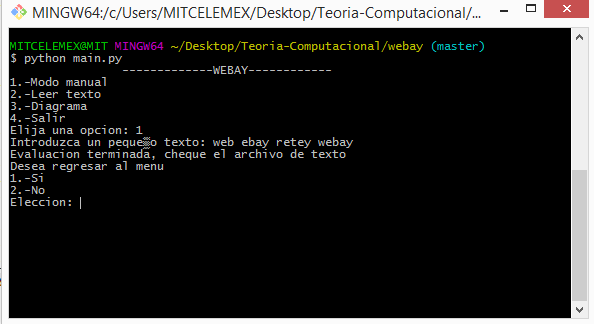
\includegraphics[width=\textwidth, height=7cm]{ModoManualWebay.png}
\label{fig:manual_webay}
\caption{Palabras de prueba: web ebay retey webay}
\end{figure}

\begin{figure}[H]
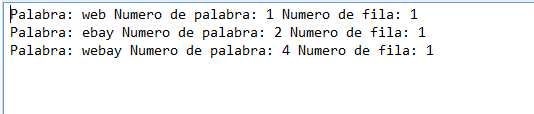
\includegraphics[width=\textwidth, height=7cm]{ArchivoWebay.png}
\label{fig:manualtexto_alfabeto}
\caption{Salida del archivo de palabras encontradas}
\end{figure}

\begin{figure}[H]
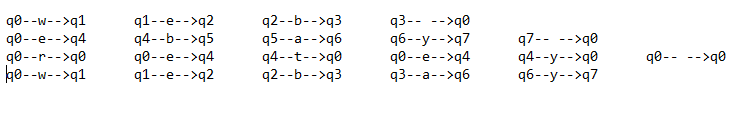
\includegraphics[width=\textwidth, height=7cm]{HistoriaWebay.png}
\label{fig:manualnuevoconteo_alfabeto}
\caption{Historia de la evaluaci\'on del aut\'omata}
\end{figure}

Para el modo de lectura de un archivo:\\
\begin{figure}[H]
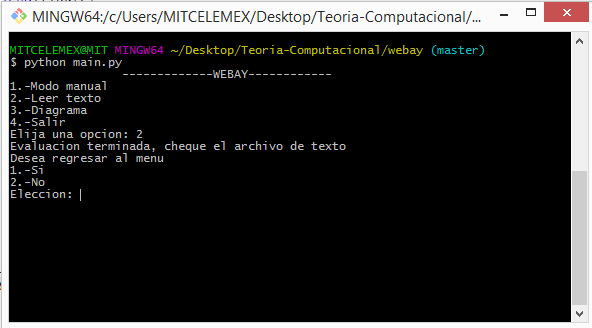
\includegraphics[width=\textwidth, height=7cm]{ModoAutomaticoWebay.png}
\label{fig:auto_alfabeto}
\caption{Lectura de un texto con palabras WEB}
\end{figure}

\begin{figure}[H]
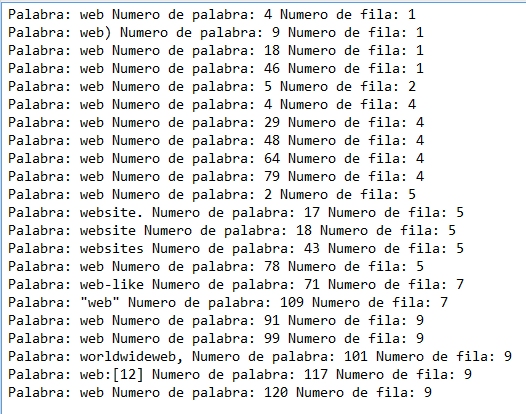
\includegraphics[width=\textwidth, height=7cm]{ArchivoTextoWebay.png}
\label{fig:autotexto_alfabeto}
\caption{Palabras encontradas del texto}
\end{figure}

\begin{figure}[H]
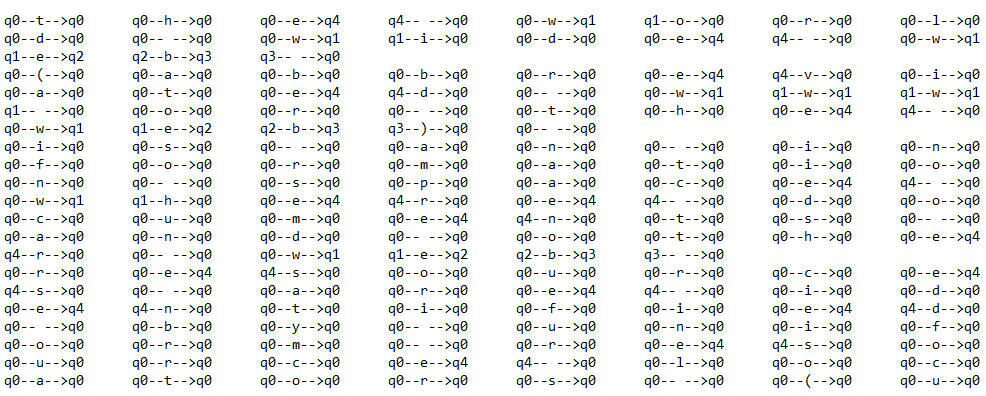
\includegraphics[width=\textwidth, height=7cm]{HistoriaWebayA.png}
\label{fig:manualnuevoconteo_alfabeto}
\caption{Historia de la evaluaci\'on del aut\'omata}
\end{figure}

%\begin{figure}[H]
%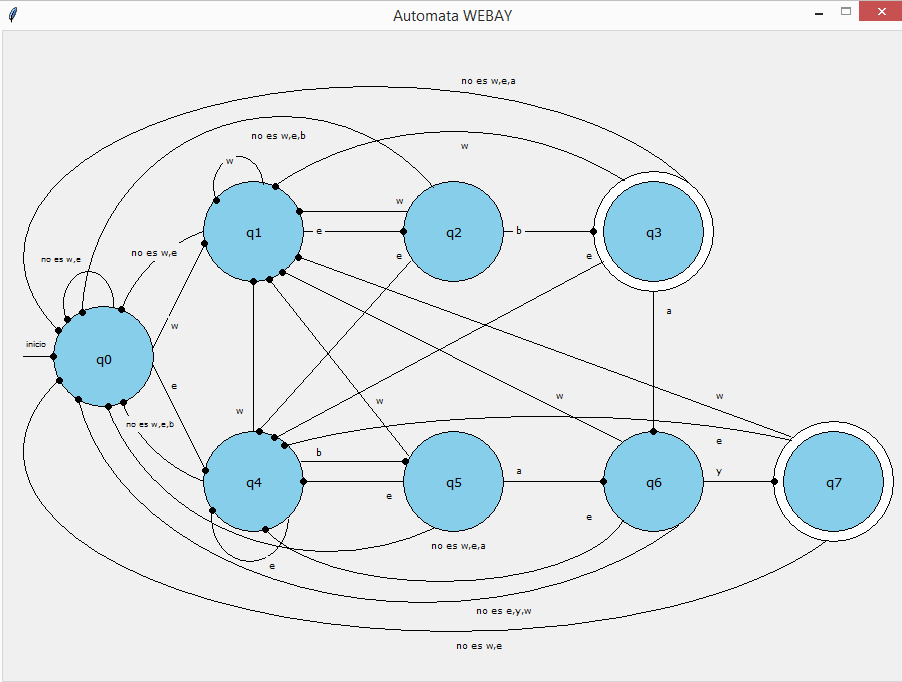
\includegraphics[width=\textwidth, height=7cm]{DiagramaWebay.png}
%\label{fig:manualnuevoconteo_alfabeto}
%\caption{Diagrama del aut\'omata}
%\end{figure}

\newpage



\section{Balanceo de Par\'entesis}
\subsection{ Descripci\'on del programa}
\justify
El siguiente programa verificar que los par\'entesis de una cadena esten balanceados, el programa tiene un modo manual, la entrada de este modo acepta todo tipo de caracteres ASCII.De igual forma cuenta con un modo autom\'atico con el cual se genera una cadena de par\'entesis aleatoria con una longitud que puede estar entre 0 y 1000.\\
En un archivo se muestra la historia que se sigui\'o al momento de hacer la evualuaci\'on de los par\'entesis, as\'i como las reglas que se utilizaron al momento de evaluar cada car\'acter.\\
\subsection{C\'odigo}
El c\'digo utilizado para la resoluci\'on del problema se muestra a continuaci\'on:\\

C\'odigo:balanceo.py

\lstset{language=Python, breaklines=true, basicstyle=\footnotesize}
\begin{lstlisting}[frame=single]
	

def VerificarBalanceo(cadena,archivo):
    exp='B'
    i=-1;
    cadena_aux=''
    archivo.write(exp)
    while True:
        try:
            i=i+1
            archivo.write('\n')
            if(cadena[i]=='('):
                cadena_aux=cadena_aux+'('
                if(exp[0]=='B'):
                    exp=exp.replace('B','RB',1)
                    cadena_aux=cadena_aux.replace('B','RB',1)
                    archivo.write(cadena_aux+exp)
                    archivo.write('\t\t\tB->(RB')
                    continue
                if(exp[0]=='R'):
                    exp=exp.replace('R','RR',1)
                    cadena_aux=cadena_aux.replace('R','RR',1)
                    archivo.write(cadena_aux+exp)
                    archivo.write('\t\t\tR->(RR')
                    continue
            if(cadena[i]==')'):
                if(exp[0]=='R'):
                    exp=exp[1:]
                    cadena_aux=cadena_aux+')'
                    archivo.write(cadena_aux+exp)
                    archivo.write('\t\t\tR-> )')
                    continue
                elif(exp[0]=='B'):
                    exp=''
                    print('Cadena no balanceada')
                    break
                else:
                    exp=''
                    continue
        except:
            if(exp=='B'):
                archivo.write(cadena_aux)
                archivo.write('\t\t\tB-> e \n')
                print('Cadena balanceada')
            else:
                print('Cadena no balanceada')
            break

\end{lstlisting}
\vspace{1.5cm}
C\'odigo:main.py

\lstset{language=Python, breaklines=true, basicstyle=\footnotesize}
\begin{lstlisting}[frame=single]
	import random
import balanceo

def IniciarArchivo():
    archivo=open("Gramatica.txt","w")
    archivo.close
def Menu():
    print("------Menu-----")
    print("1.-Modo Manual")
    print("2.-Modo Automatico")
    print("3.-Salir")
def Eleccion():
    op=input("Elige una opcion: ")
    try:
        op=int(op)
    except:
        print("Introduzca una opcion valida")
    return op
def longitud():
    lon=random.randint(1,100)
    return lon

def generarCadena():
    lon=longitud()
    cadena=''
    for c in range(1,lon+1):
        o=random.randint(1,2)
        if(o==1):
            cadena=cadena+'('
        else:
            cadena=cadena+')'
    return cadena

def Manual():
    try:
        archivo=open("Gramatica.txt","a")
    except:
        print("Error al abrir el archivo")
        exit()

    cadena=input("Introduce una cadena de parentesis: ")
    balanceo.VerificarBalanceo(cadena,archivo)

def Automatico():
    try:
        archivo=open("Gramatica.txt","a")
    except:
        print("Error al abrir el archivo")
        exit()
    cadena=generarCadena()
    print(cadena)
    balanceo.VerificarBalanceo(cadena,archivo)

def VerificarDeNuevo():
    opcion=input("Desea ingresar una nueva cadena [s/n]: ")
    return opcion
def main():
    IniciarArchivo()
    Menu()
    op=Eleccion()
    while True:
        if(op==1):
            Manual()
            while True:
                rop=VerificarDeNuevo()
                if(rop=='s'):
                    break
                elif(rop=='n'):
                    exit()
                else:
                    continue
        elif(op==2):
            Automatico()
            while True:
                rop=random.randint(1,2)
                if(rop==1):
                    break
                elif(rop==2):
                    exit()
                else:
                    continue
        elif(op==3):
            exit()
        else:
            continue

main()
\end{lstlisting}
\newpage

\subsection{Pruebas}
A continuaci\'on se mostraran algunas im\'agenes capturadas al momento de ejecutar el programa, dichas im\'agenes mostraran los resultados obtenidos.\\
\vspace{1.0cm}
Para el modo manual:\\
\begin{figure}[H]
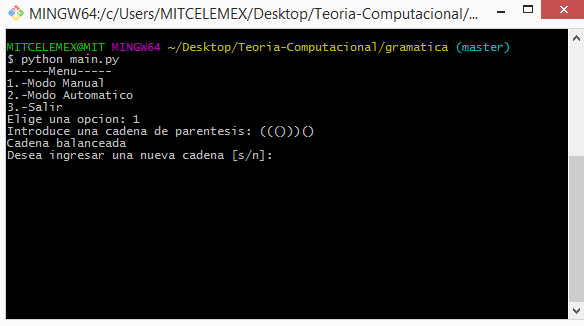
\includegraphics[width=\textwidth, height=7cm]{ModoManualPare.png}
\label{fig:manual_webay}
\caption{Cadena de par\'entesis de prueba: ((()))()}
\end{figure}

\begin{figure}[H]
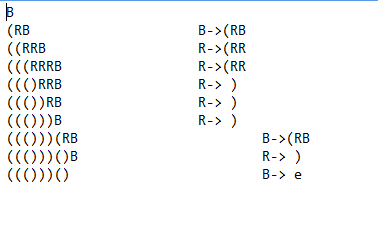
\includegraphics[width=\textwidth, height=7cm]{ArchivoPare.png}
\label{fig:manualtexto_alfabeto}
\caption{Historia de la evaluaci\'on de la cadena}
\end{figure}

Para el modo autom\'atico:\\
\begin{figure}[H]
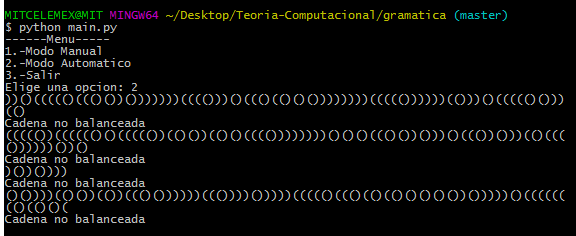
\includegraphics[width=\textwidth, height=7cm]{ModoAutomaticoPare.png}
\label{fig:auto_alfabeto}
\caption{Cadena generada autom\'aticamente}
\end{figure}

\begin{figure}[H]
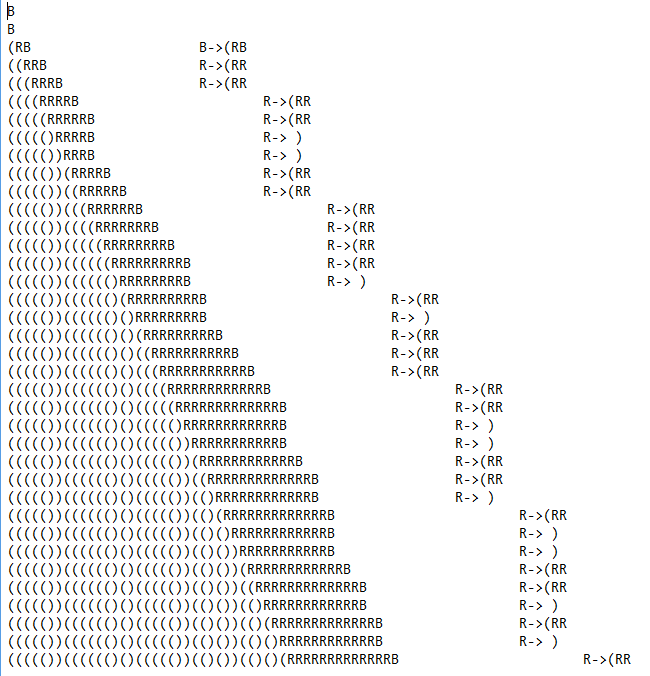
\includegraphics[width=\textwidth, height=7cm]{ArchivoHistoriaPare.png}
\label{fig:autotexto_alfabeto}
\caption{Historia de la evaluaci\'on del modo autom\'atico}
\end{figure}

\newpage


\section{Palindromos-Gram\'atica libre de contexto}
\subsection{ Descripci\'on del programa}
\justify
El siguiente programa genera palindromos de cadenas binarias, esto se logra gracias a las siguientes reglas de produccion de la gramatica:\\
\begin{center}
1.-S--$>$e\\
2.-S--$>$0\\
3.-S--$>$1\\
4.-S--$>$0S0\\
5.-S--$>$1S1\\
\end{center}
El programa cuenta con un modo manual y autom\'atico, con el cual se podr\'a elegir el tama\~no del palindromo, como salidas se obtendr\'a en un archivo la forma en que se fue generando y en otro archivo la regla que se utilizo en cada caso.
\\
\subsection{C\'odigo}
El c\'digo utilizado para la resoluci\'on del problema se muestra a continuaci\'on:\\

C\'odigo:palindromo.py

\lstset{language=Python, breaklines=true, basicstyle=\footnotesize}
\begin{lstlisting}[frame=single]
	import random;

def IniciarArchivo():
	archivo=open("palindromo.txt","w")
	archivo.close
	historia=open("historiaPal.txt","w")
	historia.close

def Run(pal,longitud,par):
	try:
		archivo=open("palindromo.txt","a")
		historia=open("historiaPal.txt","a")
	except:
		exit()
	archivo.write("S")
	exito=generar_palindromo1(archivo,pal,longitud,par,historia)
	archivo.write("\n\n")
	historia.write("------\n\n")
	archivo.close
	historia.close
	return exito

def opcion_fin(par):
	if(par==True):
		op=1
	else:
		op=random.randint(2,3)
	return op

def opcion_inicio():
	op=random.randint(4,5)
	return op

def regla1(pal,historia):
	pal=pal.replace("S","")
	historia.write("\n1.-S-->e")
	return pal

def regla2(pal,historia):
	pal=pal.replace("S",'0')
	historia.write("\n2.-S-->0")
	return pal

def regla3(pal,historia):
	pal=pal.replace("S",'1')
	historia.write("\n3.-S-->1")
	return pal

def regla4(pal,historia):
	pal=pal.replace("S","0S0")
	historia.write("\n4.-S-->0S0")
	return pal
def regla5(pal,historia):
	pal=pal.replace("S","1S1")
	historia.write("\n5.-S-->1S1")
	return pal

def generar_palindromo1(archivo,pal,longitud,par,historia):
	
	if(longitud>1):
		
		opcion=opcion_inicio()
		if(opcion==4):
			pal=regla4(pal,historia)
			archivo.write("\n"+pal)
		if(opcion==5):
			pal=regla5(pal,historia)
			archivo.write("\n"+pal)

	if(longitud==1):
		opcion=opcion_fin(par)
		if(opcion==1):
			pal=regla1(pal,historia)
			archivo.write("\n"+pal)
		if(opcion==2):
			pal=regla2(pal,historia)
			archivo.write("\n"+pal)
		if(opcion==3):
			pal=regla3(pal,historia)
			archivo.write("\n"+pal)
	if (longitud==0):
		return 1
	longitud=longitud-1
	pal=generar_palindromo1(archivo,pal,longitud,par,historia)

\end{lstlisting}
\vspace{1.5cm}
C\'odigo:main.py

\lstset{language=Python, breaklines=true, basicstyle=\footnotesize}
\begin{lstlisting}[frame=single]
import palindromo
import random

def longitud():
	x=random.randint(0,1000);
	return x

palindromo.IniciarArchivo()
def menu():
	print("-----Menu-----")
	print("1.-Modo Manual")
	print("2.-Modo Automatico")
	print("3.-Salir")

while True:
	menu()
	opcion=input("Seleccione una opcion: ")
	if(opcion=="1"):
		tamanio=input("Ingrese un tamanio de cadena: ")
		print(tamanio)
		tamanio=int(tamanio)
		if(tamanio%2==0):
			g=palindromo.Run("S",(tamanio/2)+1,True)
		else:
			tamanio=int(tamanio/2)+1
			g=palindromo.Run("S",tamanio,False)

		while True:
			try:
				seln=input("Desea regresar al menu\n1.-Si\n2.-No\n- ")
				seln=int(seln)
			except:
				exit()

			if(seln==1):
				break
			elif(seln==2):
				exit()
			else:
				continue
	elif(opcion=="2"):
		tamanio=longitud()
		print(tamanio)
		if(tamanio%2==0):
			g=palindromo.Run("S",(tamanio/2)+1,True)
		else:
			tamanio=int(tamanio/2)+1
			g=palindromo.Run("S",tamanio,False)

		while True:
			try:
				seln=input("Desea regresar al menu\n1.-Si\n2.-No\n- ")
				seln=int(seln)
			except:
				exit()

			if(seln==1):
				break
			elif(seln==2):
				exit()
			else:
				continue

	elif(opcion=="3"):
		exit()

	else:
		print("Seleccione una opcion correcta")

\end{lstlisting}
\newpage

\subsection{Pruebas}
A continuaci\'on se mostraran algunas im\'agenes capturadas al momento de ejecutar el programa, dichas im\'agenes mostraran los resultados obtenidos.\\
\vspace{1.0cm}
Para el modo manual:\\
\begin{figure}[H]
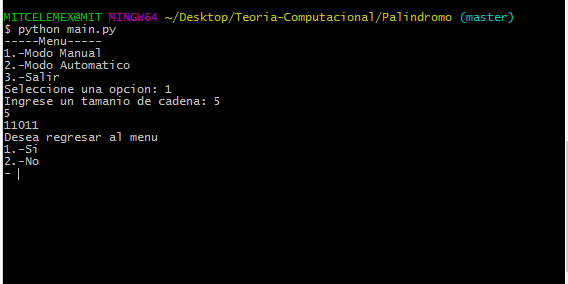
\includegraphics[width=\textwidth, height=7cm]{ModoManualPal.png}
\label{fig:manual_webay}
\caption{El tama\~no de la cadena sera de 5}
\end{figure}

\begin{figure}[H]
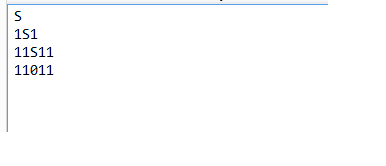
\includegraphics[width=\textwidth, height=7cm]{ArchivoPal.png}
\label{fig:manualtexto_alfabeto}
\caption{Evaluaci\'on de la gram\'atica}
\end{figure}

\begin{figure}[H]
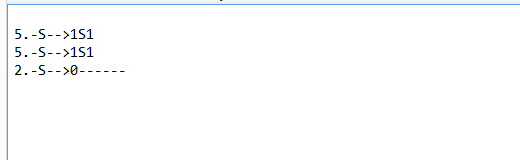
\includegraphics[width=\textwidth, height=7cm]{HistoriaPal.png}
\label{fig:manualtexto_alfabeto}
\caption{Historia de la evaluaci\'on de la gram\'atica}
\end{figure}

Para el modo autom\'atico:\\
\begin{figure}[H]
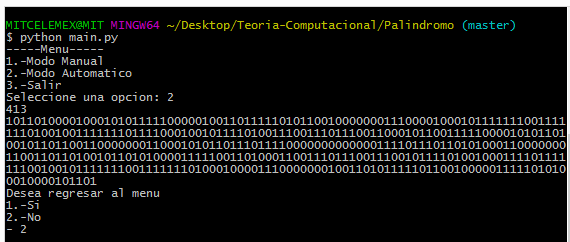
\includegraphics[width=\textwidth, height=7cm]{ModoAutomaticoPal.png}
\label{fig:auto_alfabeto}
\caption{Tama\~no generado autom\'aticamente}
\end{figure}

\begin{figure}[H]
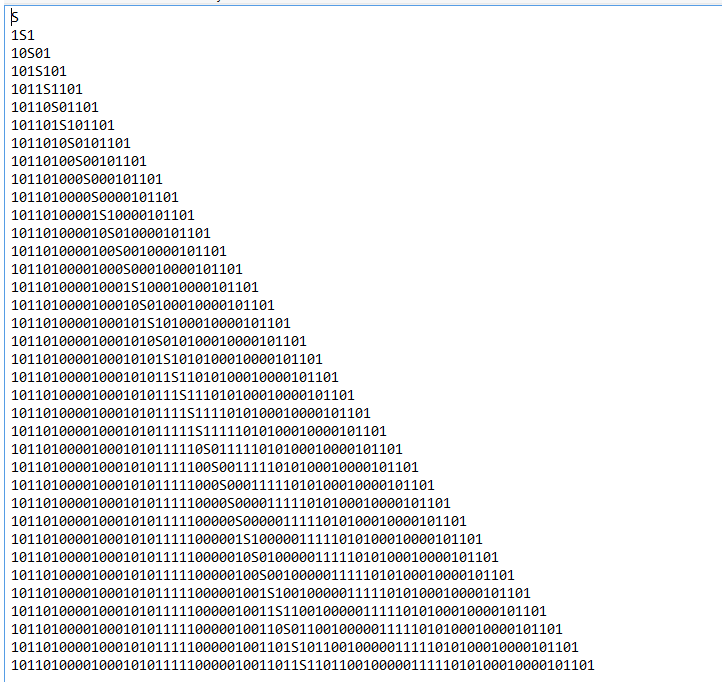
\includegraphics[width=\textwidth, height=7cm]{ArchivoHistoriaPal.png}
\label{fig:autotexto_alfabeto}
\caption{Historia de la evaluaci\'on del modo autom\'atico}
\end{figure}

\begin{figure}[H]
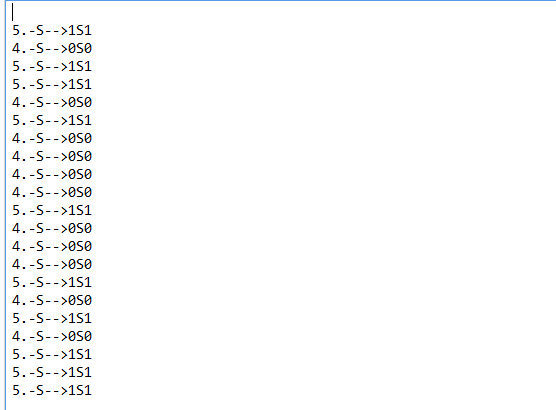
\includegraphics[width=\textwidth, height=7cm]{HistoriaPalA.png}
\label{fig:manualtexto_alfabeto}
\caption{Historia de la evaluaci\'on de la gram\'atica}
\end{figure}

\newpage

\section{Aut\'omata de Pila}
\subsection{ Descripci\'on del programa}
\justify
El siguiente programa verifica la siguiente gram\'atica $0^n 1^n$ con n $>$0, cuenta con un modo autom\'atico y manual, en la salida se imprimir\'a la historia de la evaluaci\'on de la cadena y si esta es aceptada o no,ademas se guardara de igual forma en un archivo la historia de esta misma evaluaci\'on.\\
El siguiente es un aut\'omata de pila, es decir al recibir un 0 el aut\'omata mete\'ra en la pila una X y al recibir un 1 el aut\'omata sacara esta X. La cadena ser\'a aceptada si la pila se encuentra vacia.\\
\subsection{C\'odigo}
El c\'digo utilizado para la resoluci\'on del problema se muestra a continuaci\'on:\\

C\'odigo:Nodo.java

\lstset{language=Java, breaklines=true, basicstyle=\footnotesize}
\begin{lstlisting}[frame=single]
	
package Stack;


public class Nodo {
    private String dato;
    private Nodo siguiente;

    public Nodo() {
        this.dato="";
        this.siguiente = null;
    }

  
    public String getDato() {
        return dato;
    }

    public void setDato(String dato) {
        this.dato = dato;
    }

    public Nodo getSiguiente() {
        return siguiente;
    }

    public void setSiguiente(Nodo siguiente) {
        this.siguiente = siguiente;
    }
    
    
}

\end{lstlisting}
\vspace{1.5cm}
C\'odigo:Pila.java

\lstset{language=Java, breaklines=true, basicstyle=\footnotesize}
\begin{lstlisting}[frame=single]
	
package Stack;

public class Pila {
    private Nodo tope;

    public Pila() {
        this.tope = null;
    }
    
public void push(String dato){
    Nodo nuevo = new Nodo();
    nuevo.setDato(dato);
    
    if(is_empty()){
        tope=nuevo;
    }
    else{
        nuevo.setSiguiente(tope);
        tope=nuevo;
    }
}
 
public String pop(){
    Nodo auxiliar;
    String dato="";
    if(!is_empty()){
        auxiliar=tope;
        tope=tope.getSiguiente();
        dato=auxiliar.getDato();
        auxiliar=null;
        
    }
    return dato;
}  

public boolean is_empty(){
    if(tope==null){
        return true;
    }
    else{
        return false;
    }
}

    
}

\end{lstlisting}
\vspace{1.5cm}
C\'odigo:AutomataPila.java

\lstset{language=Java, breaklines=true, basicstyle=\footnotesize}
\begin{lstlisting}[frame=single]
	
package automata;

import Stack.Pila;

import java.io.BufferedWriter;
import java.io.File;
import java.io.FileWriter;
import java.io.PrintWriter;


public class AutomataPila {
    private Pila automata;
    private int tamanio;
    private String cadena;
    
    public AutomataPila() {
        automata=new Pila();
       cadena="Z0";
    }
    
    public String evaluar(char caracter,String estado){
        //System.out.println(estado);
        if(estado.equals("q0")){
            if(caracter=='1'){
                if(!automata.is_empty()){
                    estado="q1";
                    automata.pop();
                    cadena=cadena.substring(1);
                    tamanio--;
                }
                else{
                    return "";
                }
            }
            else if(caracter=='0'){
                estado="q0";
                automata.push("X");
                cadena="X"+cadena;
                //System.out.println(automata.imprimirPila());
                tamanio++;
            }
            else{
                return "";
            }
        }
        else if(estado.equals("q1")){
            if(!automata.is_empty()){
                if(caracter=='1'){
                    estado="q1";
                    automata.pop();
                    cadena=cadena.substring(1);
                    tamanio--;
                }
                else if(caracter=='0'){
                    return "";
                }
                else{
                    return "";
                }
            
               }
            else{
                return "";
            }
        }
        return estado;
        }
   
    
    public boolean fin(){
        if(automata.is_empty()){
            return true;
        }
        else{
            return false;
        }
    }
    public void vaciarPila(){
  
        for(int i=0;i<tamanio;i++){
            automata.pop();
        }
        
        }
    
    
   public void IniciarArchivo(String texto){
    File f = new File ("archivo.txt");

        if ( !( f.exists ( ) ) ){
        try {
            FileWriter w = new FileWriter ( f, true );
            f.createNewFile ( );
            w.write (texto);
            } 
        catch ( Exception e ) {
        e.printStackTrace ( );
        }
        } 
        else {
        try{
        FileWriter w = new FileWriter ( f, true );
        w.write (texto);
        w.close ( );
        } 
        
        catch (Exception e ) {
        e.printStackTrace ( );
        }
}
   }
   

    public String getCadena() {
        return cadena;
    }

    public void setCadena(String cadena) {
        this.cadena = cadena;
    }
    
    public int GenerarNumero(){
        int numero;
        numero=(int)(Math.random()*100)+1;
        return numero;
        }
     public int Generarbit(){
        int numero;
        numero=(int)(Math.random()*2);
        return numero;
        }
   
     public String generarCadena(){
     String cadena="";
     int numero=GenerarNumero();
         for (int i = 0; i < numero; i++) {
             cadena=cadena+Generarbit();
         }
     
     return cadena;
     }
}



\end{lstlisting}
\vspace{1.5cm}
C\'odigo:main.java

\lstset{language=Java, breaklines=true, basicstyle=\footnotesize}
\begin{lstlisting}[frame=single]
	
package automata;
import java.util.Scanner;
import javax.swing.JOptionPane;


public class Main {
    
    

    public static void main(String[] args) {
       String cadena;
       String bin_aux;
       String estado="q0";
       char cadena_aux;
       AutomataPila automata=new AutomataPila();
       String opcion;
       String opcion2;
       //Menu
       
       
       System.out.println("Menu\n1.-Modo manual\n2.-Modo Automatico\n3.-Salir\nElija una opcion: ");
       Scanner entrada = new Scanner(System.in);
       opcion=entrada.nextLine();
       
       if(opcion.equals("1")){
           while(true){
                cadena=JOptionPane.showInputDialog(null,"Introduzca una cadena binaria");
                bin_aux=cadena; 
                for(int i=0;i<cadena.length();i++){
                    cadena_aux=cadena.charAt(i);
                    automata.IniciarArchivo("("+estado+", "+bin_aux+", "+automata.getCadena()+")");
                    System.out.println("("+estado+", "+bin_aux+", "+automata.getCadena()+")");
                    estado=automata.evaluar(cadena_aux,estado);
                    
                    bin_aux=bin_aux.substring(1);
                    //System.out.println(estado);
                    if(estado.equals("")){
                        break;
                    }
 
                }
                if(automata.fin() && estado.equals("q1")){
                automata.IniciarArchivo("("+estado+", e ,"+automata.getCadena()+")");
                System.out.println("("+estado+", e ,"+automata.getCadena()+")");
                estado="f";
                automata.IniciarArchivo("("+estado+", e ,"+automata.getCadena()+")\n\n");
                System.out.println("("+estado+", e ,"+automata.getCadena()+")");
                System.out.println("Cadena aceptada");
                }
                else{
                    System.out.println("Cadena no aceptada");
                }
                estado="q0";
                automata.vaciarPila();
                automata.setCadena("Z0");
                while(true){
                System.out.println("Desea evaluar otra cadena\n1.-Si\n2.-No\nElija una opcion: ");
                Scanner rentrada = new Scanner(System.in);
                opcion2=rentrada.nextLine(); 
                if(opcion2.equals("1")){
                    break;
                }
                else if(opcion2.equals("2")){
                    System.exit(0);
                    }
                }        
            }
       }         
       else if(opcion.equals("2")){
           while(true){
                cadena=automata.generarCadena();
                bin_aux=cadena;
                System.out.println(bin_aux);
                for(int i=0;i<cadena.length();i++){
                    cadena_aux=cadena.charAt(i);
                    automata.IniciarArchivo("("+estado+", "+bin_aux+", "+automata.getCadena()+")");
                    System.out.println("("+estado+", "+bin_aux+", "+automata.getCadena()+")");
                    estado=automata.evaluar(cadena_aux,estado);
                    
                    bin_aux=bin_aux.substring(1);
                    //System.out.println(estado);
                    if(estado.equals("")){
                        break;
                    }
 
                }
                if(automata.fin() && estado.equals("q1")){
                automata.IniciarArchivo("("+estado+", e ,"+automata.getCadena()+")");
                System.out.println("("+estado+", e ,"+automata.getCadena()+")");
                estado="f";
                automata.IniciarArchivo("("+estado+", e ,"+automata.getCadena()+")\n\n");
                System.out.println("("+estado+", e ,"+automata.getCadena()+")");
                System.out.println("Cadena aceptada");
                }
                else{
                    System.out.println("Cadena no aceptada");
                }
                estado="q0";
                automata.vaciarPila();
                automata.setCadena("Z0");
                while(true){
                System.out.println("Desea evaluar otra cadena\n1.-Si\n2.-No\nElija una opcion: ");
                int reop=automata.Generarbit();
                    System.out.println(reop+1);
                if(reop==0){
                    break;
                }
                else if(reop==1){
                    System.exit(0);
                    }
                }        
            }
       }
       else if(opcion.equals("3")){
           System.exit(0);
       }
       else{
           System.out.println("Opcion Invalida");
       }
       
       
       
    }
       
      
}

\end{lstlisting}

\newpage

\subsection{Pruebas}
A continuaci\'on se mostraran algunas im\'agenes capturadas al momento de ejecutar el programa, dichas im\'agenes mostraran los resultados obtenidos.\\
\vspace{1.0cm}
Para el modo manual:\\
\begin{figure}[H]
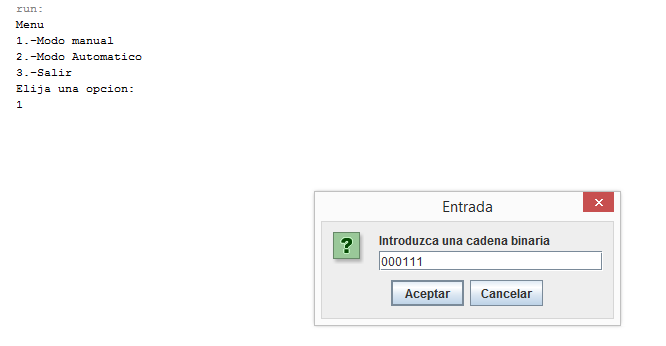
\includegraphics[width=\textwidth, height=7cm]{ModoManualPila.png}
\label{fig:manual_pila}
\caption{Cadena de prueba: 000111}
\end{figure}

\begin{figure}[H]
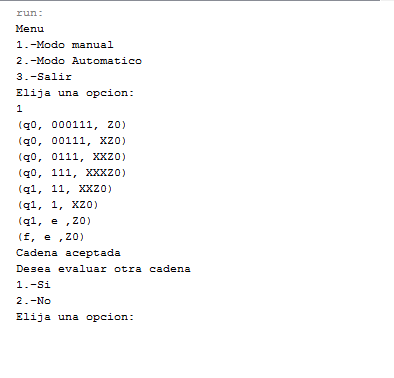
\includegraphics[width=\textwidth, height=7cm]{ModoManualPila2.png}
\label{fig:manual_pila2}
\caption{Cadena de prueba: 000111}
\end{figure}

\begin{figure}[H]
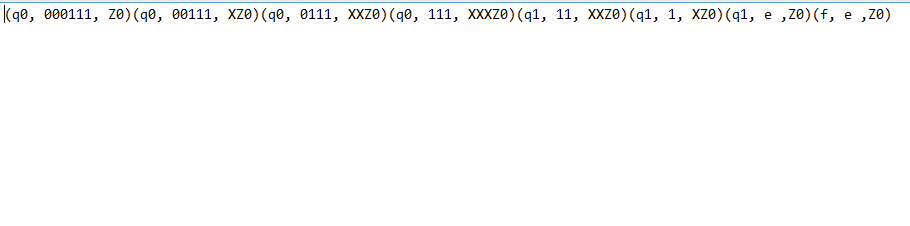
\includegraphics[width=\textwidth, height=7cm]{ArchivoPila.png}
\label{fig:manualtexto_alfabeto}
\caption{Historia de la evaluaci\'on de la cadena}
\end{figure}

Para el modo autom\'atico:\\
\begin{figure}[H]
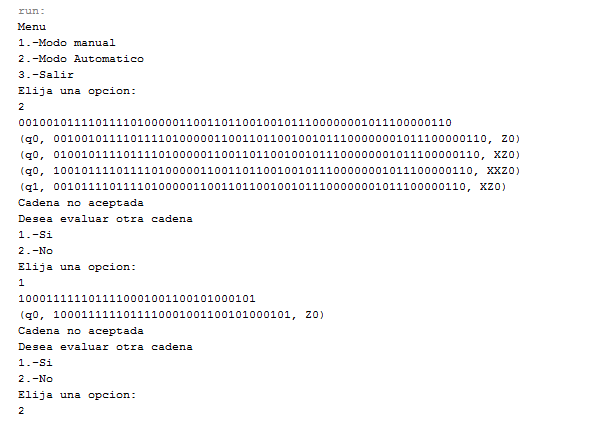
\includegraphics[width=\textwidth, height=7cm]{ModoAutomaticoPila.png}
\label{fig:auto_alfabeto}
\caption{Cadena generada autom\'aticamente}
\end{figure}

\begin{figure}[H]
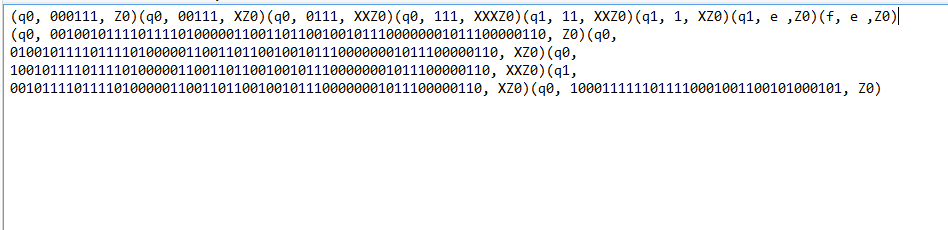
\includegraphics[width=\textwidth, height=7cm]{ArchivoHistoriaPila.png}
\label{fig:autotexto_alfabeto}
\caption{Historia de la evaluaci\'on del modo autom\'atico}
\end{figure}

\newpage


\section{Maquina de Turing}
\subsection{ Descripci\'on del programa}
\justify
El siguiente programa es la Maquina de Turing, esta evalua si una cadena cuenta con la condici\'on de ser $0^n 1^n $ con n $>=$ 1.\\
Se mostrara en un archivo de texto la forma en la que esta se evalua y como van cambiando entre sus estados, asimismo se mostrara en otro archivo las cadenas que fueron aceptadas por la maquina.\\
La maquina de Turing es la siguiente.\\

\begin{figure}[H]
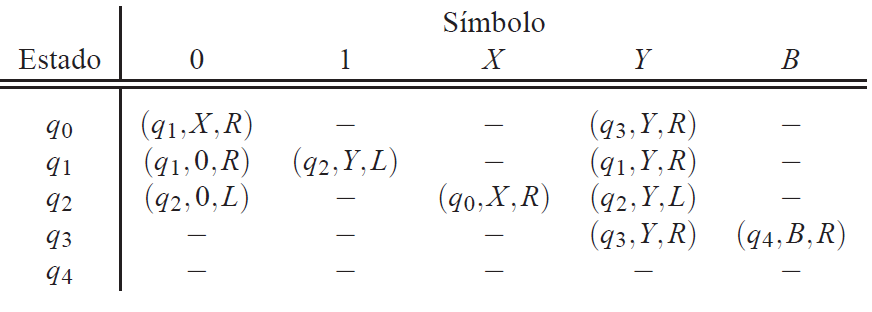
\includegraphics[width=\textwidth, height=7cm]{MT.png}
\label{fig:MT}
\caption{Maquina de Turing que acepta $0^n 1^n$ con n $>=1$}
\end{figure}

\subsection{C\'odigo}
El c\'digo utilizado para la resoluci\'on del problema se muestra a continuaci\'on:\\

C\'odigo:MaquinaTuring.py

\lstset{language=Python, breaklines=true, basicstyle=\footnotesize}
\begin{lstlisting}[frame=single]
	def maquinaTuring(cadena,archivo):
    estado=[0,"",0]
    cadena=list(cadena)
    index=0
    while True:
        for e in cadena:
            archivo.write(e)
        archivo.write("\n")
        for i in range(index):
            archivo.write(" ")
        archivo.write("|")
        archivo.write("\n")
        for i in range(index):
            archivo.write(" ")
        archivo.write("q"+str(estado[0])+"\n")
        try:
            if(index<0):
                raise Exception
            elif(estado[0]==0):
                estado[0]=estadoCero(cadena,index,estado)
                index=estado[2]
            elif(estado[0]==1):

                estado[0]=estadoUno(cadena,index,estado)
                index=estado[2]

            elif(estado[0]==2):
                estado[0]=estadoDos(cadena,index,estado)
                index=estado[2]
            elif(estado[0]==3):
                estado[0]=estadoTres(cadena,index,estado)
                index=estado[2]
            elif(estado[0]==4 or estado[0]==-1):
                break
            else:
                break
        except Exception as ex:
            if(estado[0]==3):
                estado[0]=4
            else:
                break
    return estado[0]
def estadoCero(cadena,index,estado):
    if(cadena[index]=='0'):
        cadena[index]='X'
        estado[1]="X"
        estado[2]=estado[2]+1
        return 1
    elif(cadena[index]=='Y'):
        cadena[index]='Y'
        estado[1]="Y"
        estado[2]=estado[2]+1
        return 3
    else:
        return -1

def estadoUno(cadena,index,estado):
    if(cadena[index]=='0'):
        cadena[index]='0'
        estado[1]="0"
        estado[2]=estado[2]+1
        return 1
    elif(cadena[index]=='1'):
        cadena[index]='Y'
        estado[1]="Y"
        estado[2]=estado[2]-1
        return 2
    elif(cadena[index]=='Y'):
        cadena[index]='Y'
        estado[2]=estado[2]+1
        return 1
    else:
        return -1

def estadoDos(cadena,index,estado):
    if(cadena[index]=='0'):
        cadena[index]='0'
        estado[1]="0"
        estado[2]=estado[2]-1
        return 2
    elif(cadena[index]=='X'):
        cadena[index]='X'
        estado[1]="X"
        estado[2]=estado[2]+1
        return 0
    elif(cadena[index]=='Y'):
        cadena[index]='Y'
        estado[2]=estado[2]-1
        return 2
    else:
        return -1

def estadoTres(cadena,index,estado):
    if(cadena[index]=='Y'):
        cadena[index]='Y'
        estado[1]="Y"
        estado[2]=estado[2]+1
        return 3
    elif(cadena[index]=='B'):
        cadena[index]='B'
        estado[1]="B"
        estado[2]=estado[2]+1
        return 4
    else:
        return -1

\end{lstlisting}
\vspace{1.5cm}
C\'odigo:main.py

\lstset{language=Python, breaklines=true, basicstyle=\footnotesize}
\begin{lstlisting}[frame=single]
import random
import MaquinaTuring

def longitud():
  num=random.randint(1,1000)
  return num

def num_bin():
  bin=random.randint(0,1)
  return bin

def generar_cadena():
  lon=longitud()
  cadena=''
  for i in range(1,lon+1):
    bin=str(num_bin())
    cadena=cadena+bin
  return cadena

def menu():
    print("----------------------MAQUINA DE TURING----------------------")
    print("1.-Modo Manual")
    print("2.-Modo Automatico")
    print("3.-Salir")
    op=input("Elija una opcion: ")
    return op

def iniciarArchivo():
    archivo=open("historia.txt","w")
    archivo.close
    validas=open("Validas.txt","w")
    validas.close


def manual():
    cadena=input("Ingresa una cadena binaria: ")
    return cadena

def main():
    iniciarArchivo()
    estado=[0,'',0]
    try:
        archivo=open("historia.txt","a")
        validas=open("Validas.txt","a")
    except:
        print("Error al abrir el archivo")
    while True:
        opcion=menu()
        if(opcion=='1'):
            while True:
                cadena=manual()
                estado=MaquinaTuring.maquinaTuring(cadena,archivo)
                if(estado==4):
                    validas.write(cadena)
                    validas.write("\n")
                    print("Cadena Valida")
                else:
                    print("Cadena invalida")
                while True:
                    print("Desea evaluar otra cadena [s/n]: ")
                    reop=input("")
                    if(reop=='s'):
                        break
                    if(reop=='n'):
                        exit()
        elif(opcion=='2'):
            while True:
                cadena=generar_cadena()
                estado=MaquinaTuring.maquinaTuring(cadena,archivo)
                if(estado==4):
                    validas.write(cadena)
                    validas.write("\n")
                    print("Cadena Valida")
                else:
                    print("Cadena invalida")
                archivo.write("\n\n")
                while True:
                    print("Desea regresar al menu [s/n]: ")
                    reop=num_bin()
                    if(reop==0):
                        print("s")
                        break
                    if(reop==1):
                        print('n')
                        exit()
        elif(opcion=='3'):
            archivo.close
            validas.close
            exit()
        else:
            print("Selecciona una opcion correcta")
    archivo.close
    validas.close

main()


\end{lstlisting}
\newpage

\subsection{Pruebas}
A continuaci\'on se mostraran algunas im\'agenes capturadas al momento de ejecutar el programa, dichas im\'agenes mostraran los resultados obtenidos.\\
\vspace{1.0cm}
Para el modo manual:\\
\begin{figure}[H]
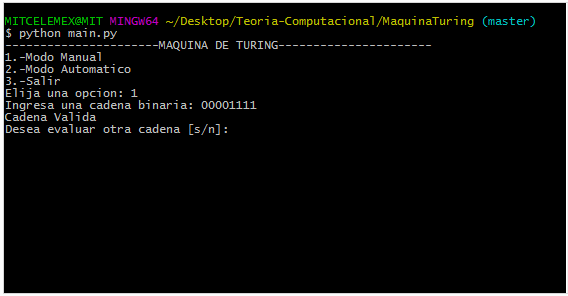
\includegraphics[width=\textwidth, height=7cm]{ModoManualTuring.png}
\label{fig:manual_webay}
\caption{La cadena a evaluar ser\'a 00001111}
\end{figure}

\begin{figure}[H]
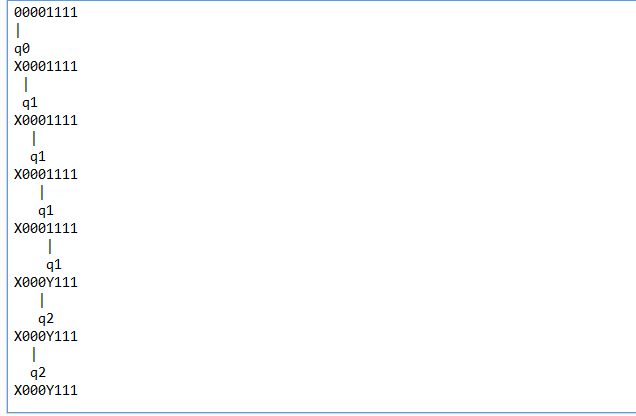
\includegraphics[width=\textwidth, height=7cm]{ArchivoTuring.png}
\label{fig:manualtexto_alfabeto}
\caption{Fragmento de la evaluaci\'on de la Maquina de Turing}
\end{figure}

Para el modo autom\'atico:\\
\begin{figure}[H]
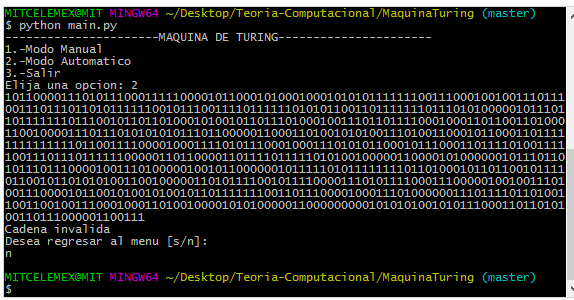
\includegraphics[width=\textwidth, height=7cm]{ModoAutomaticoTuring.png}
\label{fig:auto_alfabeto}
\caption{Tama\~no y cadena generado autom\'aticamente}
\end{figure}

\begin{figure}[H]
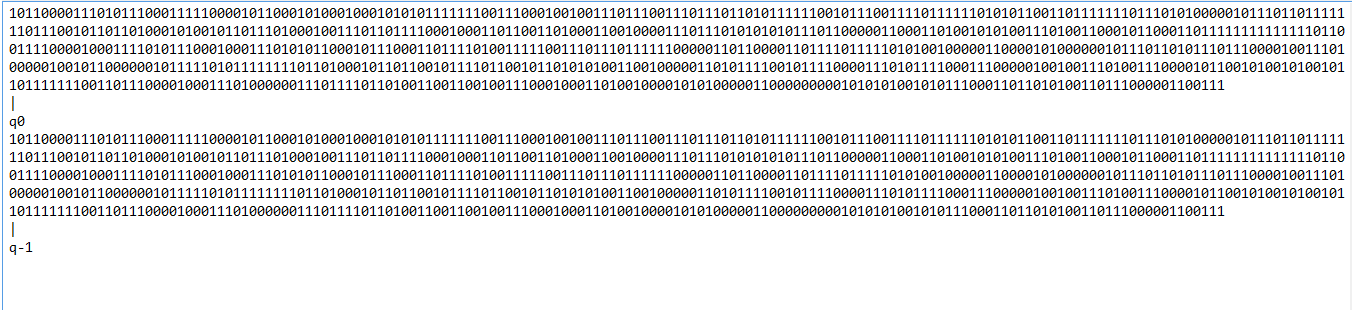
\includegraphics[width=\textwidth, height=7cm]{ArchivoHistoriaTuring.png}
\label{fig:autotexto_alfabeto}
\caption{Historia de la evaluaci\'on del modo autom\'atico}
\end{figure}

\begin{figure}[H]
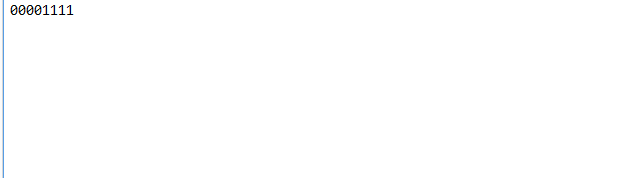
\includegraphics[width=\textwidth, height=7cm]{ValidasTuring.png}
\label{fig:manualtexto_alfabeto}
\caption{Cadenas validas aceptadas}
\end{figure}

\newpage

\end{document}